\documentclass[11pt,a4paper]{article}

% --- PAQUETES DE IDIOMA Y CODIFICACIÓN ---
\usepackage[utf8]{inputenc}
\usepackage[T1]{fontenc}
\usepackage[spanish,es-tabla,es-nodecimaldot,es-noshorthands]{babel}

% --- MATEMÁTICAS Y SÍMBOLOS ---
\usepackage{amsmath,amssymb,amsfonts}
\usepackage{mathtools}

% --- FORMATO Y DISEÑO DE PÁGINA ---
\usepackage[top=2.5cm, bottom=2.5cm, left=2.5cm, right=2.5cm]{geometry}
\usepackage{fancyhdr}
\usepackage{booktabs}
\usepackage{array}
\usepackage{enumitem}
\usepackage{titlesec}
\usepackage{graphicx}

% --- COLORES Y CÓDIGO ---
\usepackage[table]{xcolor}
\definecolor{pujblue}{RGB}{0, 51, 102}
\definecolor{darkblue}{RGB}{16, 44, 87}
\definecolor{codebg}{RGB}{248, 249, 250}
\definecolor{darkgray}{RGB}{60, 60, 60}

\usepackage{listings}
\usepackage[colorlinks=true, linkcolor=pujblue, citecolor=pujblue, urlcolor=pujblue]{hyperref}

% --- CONFIGURACIÓN DE LISTINGS ---
\lstset{
    language=Python,
    backgroundcolor=\color{codebg},
    basicstyle=\ttfamily\footnotesize,
    keywordstyle=\color{pujblue}\bfseries,
    commentstyle=\color{gray}\itshape,
    stringstyle=\color{teal},
    breaklines=true,
    frame=single,
    rulecolor=\color{black!20},
    numbers=left,
    numberstyle=\tiny\color{gray},
    numbersep=8pt,
    tabsize=4,
    showstringspaces=false,
    literate=
      {á}{{\'a}}1 {é}{{\'e}}1 {í}{{\'i}}1 {ó}{{\'o}}1 {ú}{{\'u}}1
      {Á}{{\'A}}1 {É}{{\'E}}1 {Í}{{\'I}}1 {Ó}{{\'O}}1 {Ú}{{\'U}}1
      {ñ}{{\~n}}1 {Ñ}{{\~N}}1 {ü}{{\"u}}1 {Ü}{{\"U}}1
      {¿}{{?`}}1 {¡}{{!`}}1
}

% --- ENCABEZADOS Y PIES DE PÁGINA ---
\pagestyle{fancy}
\fancyhf{}
\fancyhead[L]{\small\color{darkgray}\textit{Computación Científica}}
\fancyhead[R]{\small\color{darkgray}\textit{Taller: Interpolación y Mínimos Cuadrados}}
\fancyfoot[C]{\thepage}
\renewcommand{\headrulewidth}{0.4pt}
\renewcommand{\footrulewidth}{0.4pt}

\titleformat{\section}{\Large\bfseries\color{pujblue}}{\thesection}{1em}{}[\titlerule]
\titleformat{\subsection}{\large\bfseries\color{darkblue}}{\thesubsection}{1em}{}
\titleformat{\subsubsection}{\normalsize\bfseries\color{darkblue}}{\thesubsubsection}{1em}{}

% ==============================================================================
% INICIO DEL DOCUMENTO
% ==============================================================================
\begin{document}

\begin{center}
    {\LARGE\bfseries\color{pujblue} Taller: Interpolación y Mínimos Cuadrados}\\[0.3cm]
    {\large Computación Científica --- Pontificia Universidad Javeriana Cali}\\[0.1cm]
    {\normalsize Profesor: Juan Fernando Paz}\\[0.1cm]
    {\normalsize Estudiante: Miguel Angel Padilla Rosero}
\end{center}
\vspace{0.3cm}

% ==============================================================================
% CÓDIGO BASE EN PYTHON
% ==============================================================================
\section{Implementación de los Algoritmos Base en Python}

Para resolver el taller se implementaron los métodos de interpolación de Lagrange y de ajuste por mínimos cuadrados usando ecuaciones normales y factorización QR:

\begin{lstlisting}
import numpy as np

def interpolar_lagrange(t_nodos, y_nodos, t_eval):
    n = len(t_nodos)
    resultado = 0.0
    for i in range(n):
        L_i = 1.0
        for j in range(n):
            if i != j:
                L_i *= (t_eval - t_nodos[j]) / (t_nodos[i] - t_nodos[j])
        resultado += y_nodos[i] * L_i
    return resultado

def ajuste_polinomial(x, y, grado):
    # Matriz de Vandermonde con potencias crecientes
    A = np.vander(x, N=grado + 1, increasing=True)
    
    # Metodo 1: Ecuaciones Normales
    c_NE = np.linalg.solve(A.T @ A, A.T @ y)
    
    # Metodo 2: Factorizacion QR
    Q, R = np.linalg.qr(A)
    c_QR = np.linalg.solve(R, Q.T @ y)
    
    return c_NE, c_QR, A
\end{lstlisting}

% ==============================================================================
% EJERCICIO 1
% ==============================================================================
\section{Ejercicio 1: Interpolación de Datos}

Se tienen las siguientes mediciones experimentales de la posición de un objeto en el tiempo:

\begin{table}[h!]
    \centering
    \caption{Datos experimentales de posición vs. tiempo.}
    \begin{tabular}{ccccc}
        \toprule
        $t$ & $0$ & $1$ & $2$ & $3$ \\
        \midrule
        $x(t)$ & $1.0$ & $2.7$ & $5.8$ & $10.9$ \\
        \bottomrule
    \end{tabular}
\end{table}

\subsection{a) Grado máximo del polinomio interpolante}
Al tener 4 puntos $(t_i, x(t_i))$ con tiempos distintos, el polinomio interpolante tiene como grado máximo $n = 3$ (grado cúbico). Con 4 puntos, la matriz de Vandermonde es cuadrada de $4 \times 4$ y su determinante es distinto de cero, lo que asegura que existe un único polinomio de grado menor o igual a 3 que pasa por todos los puntos.

\subsection{b) y c) Polinomios de Lagrange $L_i(t)$}
Calculamos cada término usando la fórmula $L_i(t) = \prod_{j \neq i} \frac{t - t_j}{t_i - t_j}$:
\begin{align*}
    L_0(t) &= \frac{(t-1)(t-2)(t-3)}{(0-1)(0-2)(0-3)} = -\frac{1}{6}t^3 + t^2 - \frac{11}{6}t + 1 \\
    L_1(t) &= \frac{t(t-2)(t-3)}{(1-0)(1-2)(1-3)} = \frac{1}{2}t^3 - \frac{5}{2}t^2 + 3t \\
    L_2(t) &= \frac{t(t-1)(t-3)}{(2-0)(2-1)(2-3)} = -\frac{1}{2}t^3 + 2t^2 - \frac{3}{2}t \\
    L_3(t) &= \frac{t(t-1)(t-2)}{(3-0)(3-1)(3-2)} = \frac{1}{6}t^3 - \frac{1}{2}t^2 + \frac{1}{3}t
\end{align*}

\subsection{d) Expresión simplificada de $p(t)$}
Multiplicamos cada polinomio base por su valor correspondiente $x(t_i)$:
\begin{equation}
    p(t) = 1.0\,L_0(t) + 2.7\,L_1(t) + 5.8\,L_2(t) + 10.9\,L_3(t)
\end{equation}
Agrupando potencias semejantes:
\begin{equation}
    p(t) = 0.1\,t^3 + 0.4\,t^2 + 1.2\,t + 1.0 = \frac{1}{10}t^3 + \frac{2}{5}t^2 + \frac{6}{5}t + 1
\end{equation}

\subsection{e) y f) Estimaciones de posición en $t = 1.5$ y $t = 2.5$}
Evaluamos el polinomio directamente en los puntos requeridos:
\begin{itemize}[leftmargin=*]
    \item Para $t = 1.5$: \quad $p(1.5) = 0.1(1.5)^3 + 0.4(1.5)^2 + 1.2(1.5) + 1.0 = 4.0375\text{ m}$.
    \item Para $t = 2.5$: \quad $p(2.5) = 0.1(2.5)^3 + 0.4(2.5)^2 + 1.2(2.5) + 1.0 = 8.0625\text{ m}$.
\end{itemize}

\subsection{g) Verificación computacional}
Evaluando el polinomio en los 4 instantes originales:
\begin{align*}
    p(0) &= 1.0 \quad (\text{diferencia } = 0.0) \\
    p(1) &= 0.1(1) + 0.4(1) + 1.2(1) + 1.0 = 2.7 \quad (\text{diferencia } = 0.0) \\
    p(2) &= 0.1(8) + 0.4(4) + 1.2(2) + 1.0 = 5.8 \quad (\text{diferencia } = 0.0) \\
    p(3) &= 0.1(27) + 0.4(9) + 1.2(3) + 1.0 = 10.9 \quad (\text{diferencia } = 0.0)
\end{align*}
El polinomio pasa de forma exacta por los 4 datos de la tabla.

\subsection{h) Ajuste con polinomios de grado 4 o superior}
Si usamos un polinomio de grado 4 o mayor, tendríamos 5 o más coeficientes para solo 4 datos. Esto hace que el sistema sea subdeterminado, por lo que existen infinitos polinomios distintos que pasan por esos mismos 4 puntos. Si intentamos resolverlo por mínimos cuadrados sin regularización, la matriz $A^T A$ no tendría rango completo y sería singular (no se puede invertir). Además, aumentar el grado sin necesidad genera sobreajuste, produciendo oscilaciones irreales entre los puntos y divergencia fuera del intervalo $[0, 3]$.

\begin{figure}[h!]
    \centering
    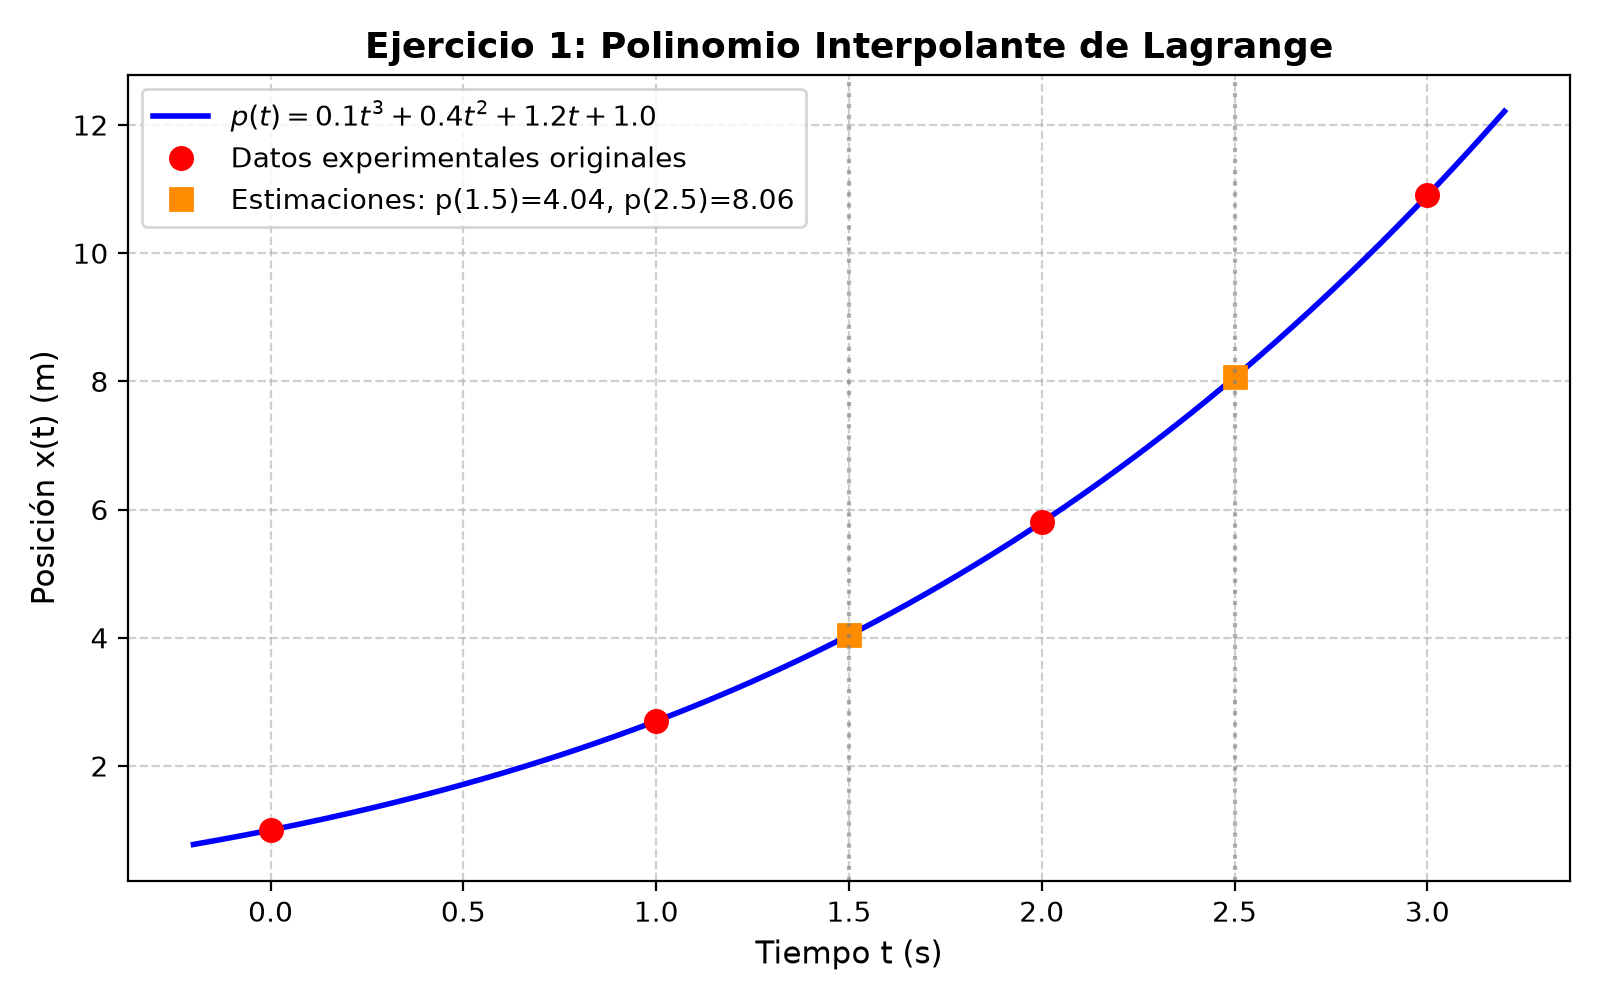
\includegraphics[width=0.68\textwidth]{fig_ejercicio1_lagrange.png}
    \caption{Curva interpolante $p(t)$ junto con los datos y estimaciones.}
\end{figure}

% ==============================================================================
% EJERCICIO 2
% ==============================================================================
\section{Ejercicio 2: Interpolación y Polinomio de Taylor}

Se analiza la función $f(x) = \frac{1}{1 + x^2}$ alrededor de $x_0 = 0$.

\subsection{Parte A. Polinomio de Taylor}
Derivando $f(x) = (1+x^2)^{-1}$ y evaluando en $x_0 = 0$:
\[
    f(0) = 1, \quad f'(0) = 0, \quad f''(0) = -2, \quad f'''(0) = 0, \quad f^{(4)}(0) = 24, \quad f^{(6)}(0) = -720
\]
Esto también se deduce directamente de la serie geométrica $\frac{1}{1 - (-x^2)} = 1 - x^2 + x^4 - x^6 + \dots$ para $|x| < 1$. Por lo tanto, los polinomios de Taylor son:
\begin{itemize}[leftmargin=*]
    \item $T_2(x) = 1 - x^2$
    \item $T_4(x) = 1 - x^2 + x^4$
    \item $T_6(x) = 1 - x^2 + x^4 - x^6$
\end{itemize}

\begin{figure}[h!]
    \centering
    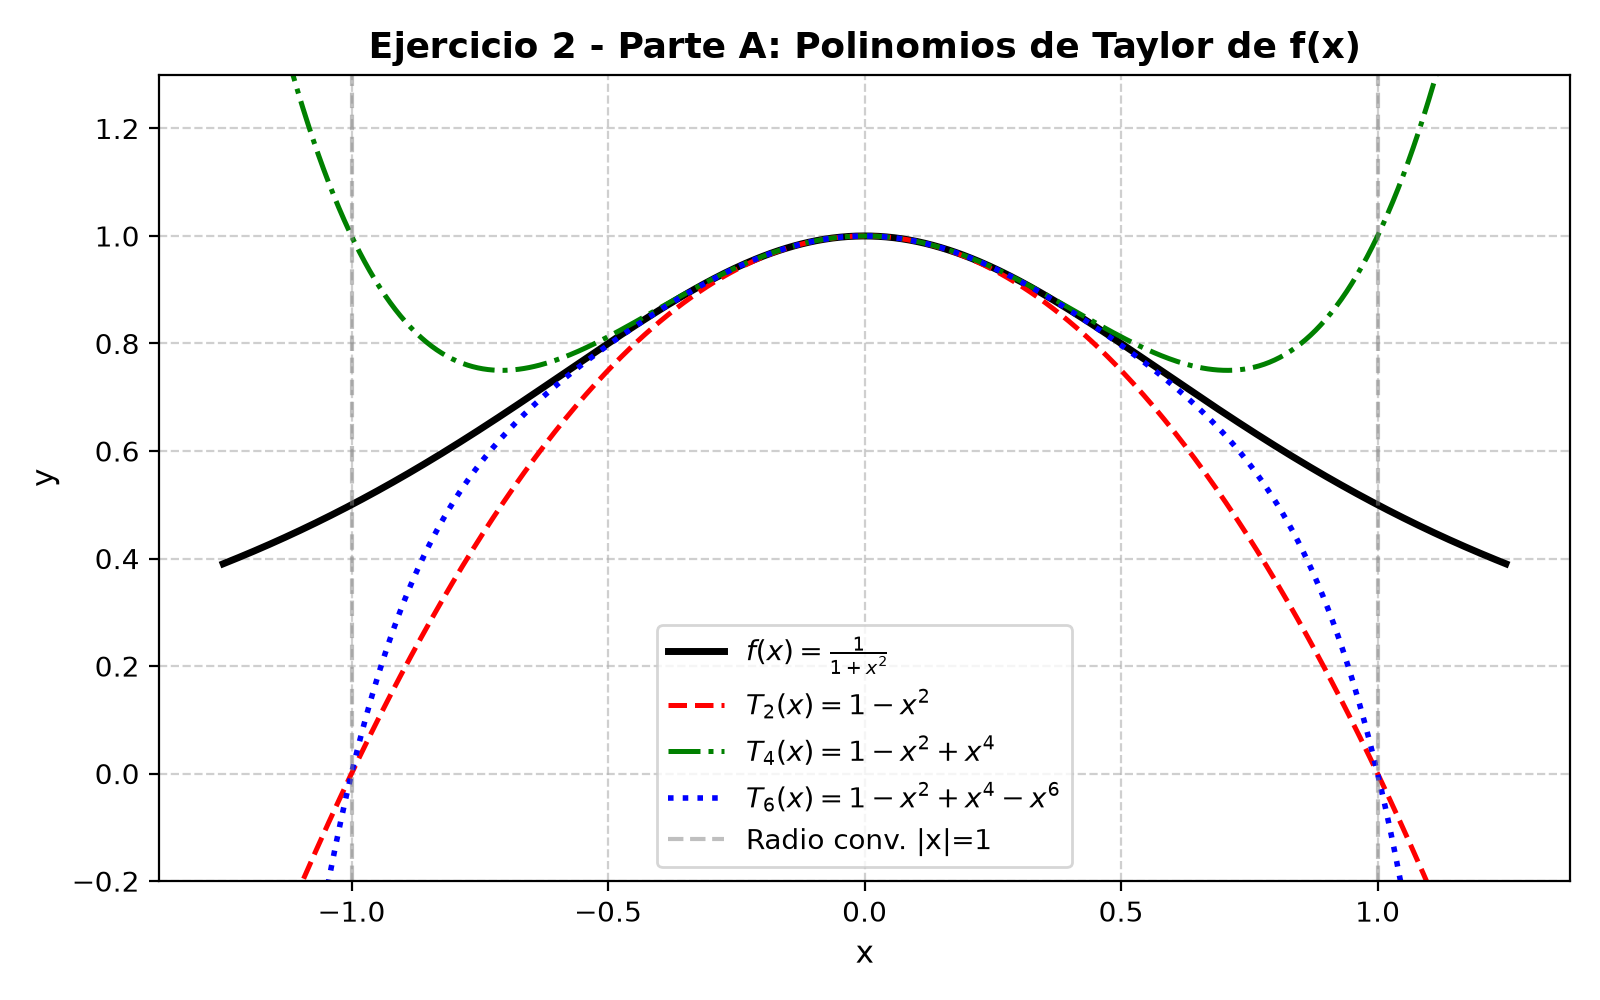
\includegraphics[width=0.68\textwidth]{fig_ejercicio2_taylor.png}
    \caption{Función $f(x)$ junto a sus polinomios de Taylor.}
\end{figure}

\subsection{Parte B. Polinomio interpolante}
Tomando los puntos $x_i \in \{-1, -0.5, 0, 0.5, 1\}$, los valores correspondientes son:
\[
    y_0 = 0.5, \quad y_1 = 0.8, \quad y_2 = 1.0, \quad y_3 = 0.8, \quad y_4 = 0.5
\]
Como la función y los puntos son pares, los coeficientes de potencias impares son cero, quedando $p(x) = c_4 x^4 + c_2 x^2 + c_0$. Al resolver el sistema de interpolación se obtiene:
\begin{equation}
    p(x) = 0.4\,x^4 - 0.9\,x^2 + 1.0 = \frac{2}{5}x^4 - \frac{9}{10}x^2 + 1
\end{equation}
Verificamos que coincide en todos los puntos: $p(0) = 1.0$, $p(\pm 0.5) = 0.8$ y $p(\pm 1) = 0.5$.

\begin{figure}[h!]
    \centering
    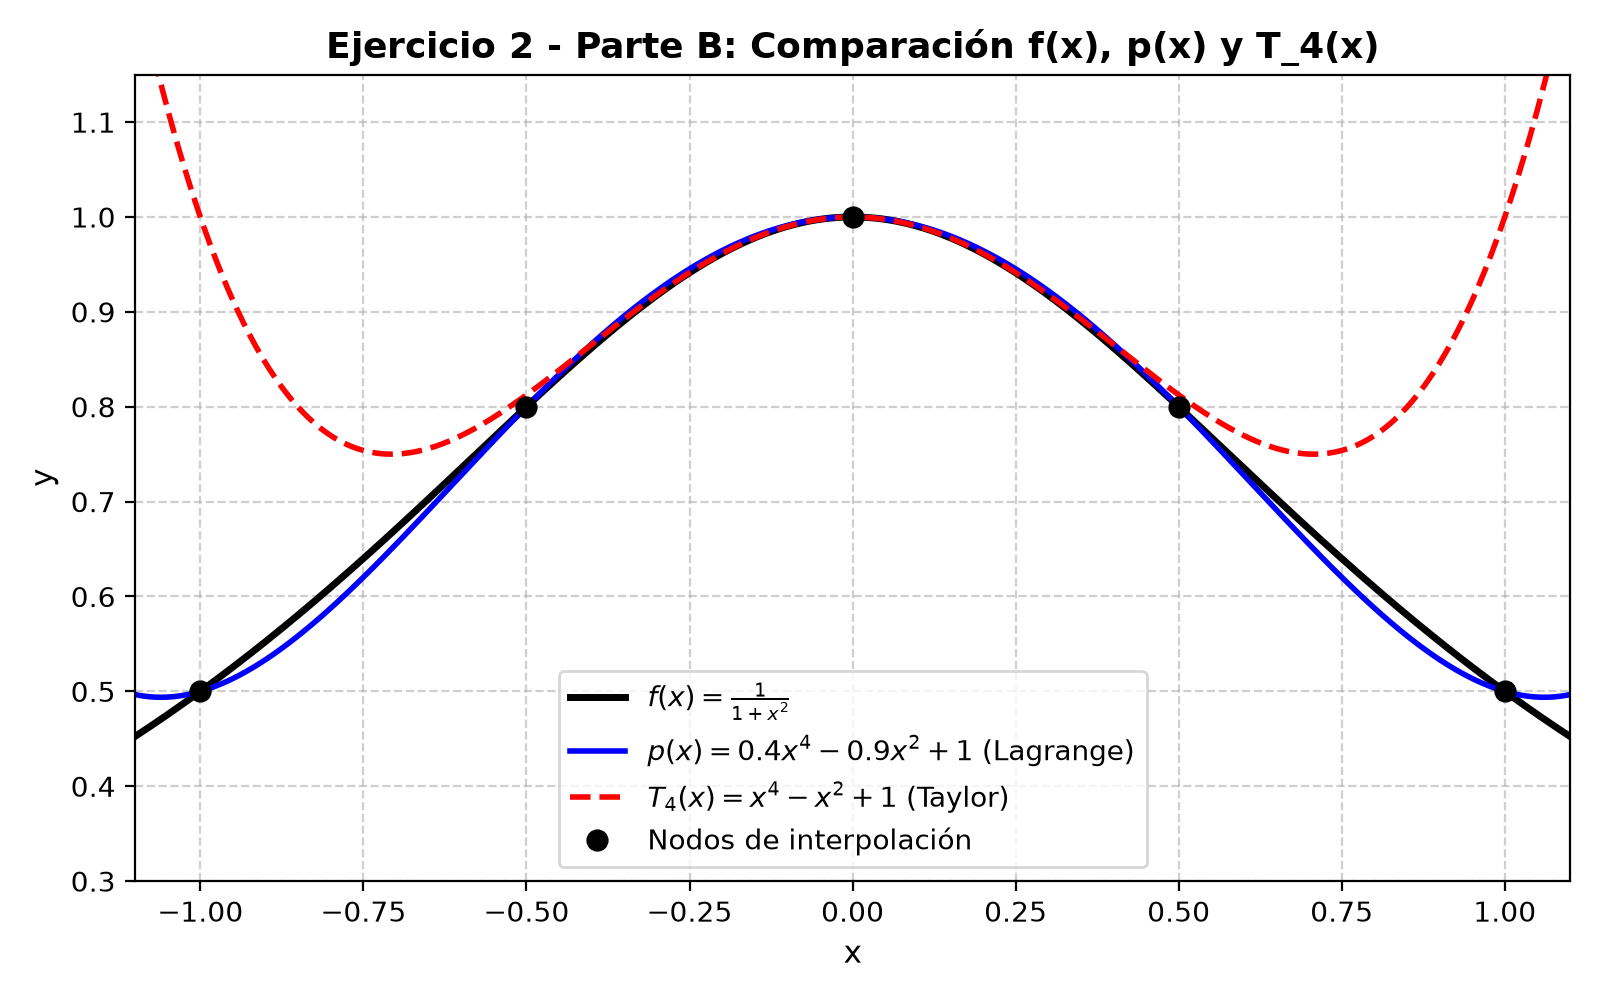
\includegraphics[width=0.68\textwidth]{fig_ejercicio2_comparacion.png}
    \caption{Comparación entre $f(x)$, interpolación $p(x)$ y Taylor $T_4(x)$.}
\end{figure}

\subsection{Parte C. Comparación de errores en $[-1, 1]$}
Calculamos los errores absolutos $e_p(x) = |f(x) - p(x)|$ y $e_T(x) = |f(x) - T_4(x)|$:
\begin{itemize}[leftmargin=*]
    \item El error máximo de Taylor en $[-1, 1]$ es $0.5000$ (ocurre en los extremos $x = \pm 1$).
    \item El error máximo de interpolación es $0.0223$ (ocurre cerca de $x \approx \pm 0.83$).
    \item El error máximo de Taylor es aproximadamente 22 veces mayor que el de la interpolación.
\end{itemize}

\begin{table}[h!]
    \centering
    \caption{Evaluación en los puntos solicitados.}
    \begin{tabular}{cccccc}
        \toprule
        $x$ & $f(x)$ & $T_4(x)$ & $|f(x) - T_4(x)|$ & $p(x)$ & $|f(x) - p(x)|$ \\
        \midrule
        $0.1$ & $0.990099$ & $0.990100$ & $9.90 \times 10^{-7}$ & $0.991040$ & $9.41 \times 10^{-4}$ \\
        $0.5$ & $0.800000$ & $0.812500$ & $1.25 \times 10^{-2}$ & $0.800000$ & $0.00$ \\
        $1.0$ & $0.500000$ & $1.000000$ & $5.00 \times 10^{-1}$ & $0.500000$ & $0.00$ \\
        \bottomrule
    \end{tabular}
\end{table}

Cerca de $0$ ($|x| \le 0.3$), Taylor es mucho más preciso, con un error cercano a $10^{-6}$ en $x = 0.1$. Sin embargo, al alejarnos hacia los bordes, el error de Taylor crece rápidamente y en $x = 1.0$ llega al $50\%$. Esto se debe a que en el plano complejo $f(z) = \frac{1}{1+z^2}$ tiene polos en $z = \pm i$, por lo que su radio de convergencia es $R = 1$. Cerca de ese límite, la serie de Taylor pierde precisión. En cambio, la interpolación distribuye nodos en todo el intervalo $[-1, 1]$, fijando la función en los extremos y manteniendo un error pequeño en toda la región.

\subsection{Parte D. Taylor e Interpolación}
\begin{enumerate}[label=\alph*), leftmargin=*]
    \item El polinomio de Taylor utiliza información local en un único punto $x_0$ (el valor de la función y sus derivadas sucesivas en ese punto).
    \item El polinomio interpolante utiliza información distribuida, es decir, parejas $(x_i, y_i)$ repartidas en varios puntos del dominio.
    \item No, para interpolar no se necesitan derivadas, únicamente conocer los valores de la función en los nodos.
    \item No, para Taylor no se necesitan varios puntos; todo el polinomio se construye a partir de lo que ocurre en $x_0$.
    \item Es una aproximación local porque busca contacto de orden superior en $x_0$ (mismo valor y mismas derivadas). Por esa razón, su precisión decae a medida que nos alejamos del punto central.
    \item La interpolación es distribuida porque obliga al polinomio a cruzar por los nodos fijados en distintos puntos del intervalo, repartiendo el error a lo largo del dominio.
\end{enumerate}

\paragraph{Pregunta de cierre:}
Tiene sentido usar Taylor cuando se conoce la función analítica y sus derivadas, y se quiere aproximar el comportamiento en un entorno pequeño alrededor de un punto de interés (por ejemplo en física o para linealizar un sistema). Por el contrario, tiene sentido usar interpolación cuando los datos vienen de experimentos o tablas (donde no hay derivadas disponibles), o cuando se requiere una buena aproximación en todo un intervalo amplio.

% ==============================================================================
% EJERCICIO 3
% ==============================================================================
\section{Ejercicio 3: Mínimos Cuadrados y Matrices Mal Condicionadas}

Se tienen 50 mediciones $(x_i, y_i)$ con $x \in [0.00, 0.98]$ en pasos de $0.02$. Se ajusta un polinomio de grado 12 con coeficientes $c_0, c_1, \dots, c_{12}$. La matriz de Vandermonde $A$ tiene dimensión $50 \times 13$.

\subsection{a) y b) Coeficientes y residuos}
Resolvemos el ajuste por dos vías: Ecuaciones Normales ($A^T A c = A^T y$) y Factorización QR ($R c = Q^T y$):

\begin{table}[h!]
    \centering
    \caption{Comparación de coeficientes entre Ecuaciones Normales y QR.}
    \begin{tabular}{crrr}
        \toprule
        Coeficiente & Ecuaciones Normales (NE) & Factorización QR & Diferencia \\
        \midrule
        $c_0$   & $1.022229$        & $1.019097$        & $3.13 \times 10^{-3}$ \\
        $c_1$   & $-0.411199$       & $0.884826$        & $1.30 \times 10^{0}$ \\
        $c_2$   & $77.831111$       & $18.947488$       & $5.89 \times 10^{1}$ \\
        $c_3$   & $-1\,138.064095$  & $-92.222880$      & $1.05 \times 10^{3}$ \\
        $c_4$   & $9\,354.302028$   & $-363.736624$     & $9.72 \times 10^{3}$ \\
        $c_5$   & $-47\,242.459426$ & $6\,641.245578$   & $5.39 \times 10^{4}$ \\
        $c_6$   & $156\,079.372309$ & $-35\,008.421078$ & $1.91 \times 10^{5}$ \\
        $c_7$   & $-348\,220.950968$& $100\,939.708839$ & $4.49 \times 10^{5}$ \\
        $c_8$   & $528\,862.697675$ & $-179\,212.947340$& $7.08 \times 10^{5}$ \\
        $c_9$   & $-538\,892.148505$& $201\,505.998301$ & $7.40 \times 10^{5}$ \\
        $c_{10}$& $352\,392.748589$& $-140\,231.222729$& $4.93 \times 10^{5}$ \\
        $c_{11}$& $-133\,570.609509$& $55\,232.406639$ & $1.89 \times 10^{5}$ \\
        $c_{12}$& $22\,300.729370$ & $-9\,427.640971$  & $3.17 \times 10^{4}$ \\
        \bottomrule
    \end{tabular}
\end{table}

Calculando la norma del vector residuo $r = y - Ac$:
\begin{align*}
    \|r_{\text{NE}}\|_2 &= 0.04928570 \\
    \|r_{\text{QR}}\|_2 &= 0.04689452 \\
    \text{Diferencia} &= 2.39 \times 10^{-3}
\end{align*}
Los coeficientes difieren en valores enormes (de hasta $7.4 \times 10^5$), pero las normas de los residuos son casi idénticas, con una diferencia de apenas $0.0024$.

\subsection{c) y d) Gráfica y evaluación en $[0, 1]$}
Evaluamos ambos modelos en una malla uniforme de 1000 puntos en $[0, 1]$:
\begin{itemize}[leftmargin=*]
    \item La diferencia máxima entre ambas curvas en el intervalo es de $0.0405$.
    \item La diferencia promedio es de $0.0021$.
    \item En el extremo $x = 1.0$: $p_{\text{NE}}(1.0) = 4.0596$ frente a $p_{\text{QR}}(1.0) = 4.0191$.
\end{itemize}

\begin{figure}[h!]
    \centering
    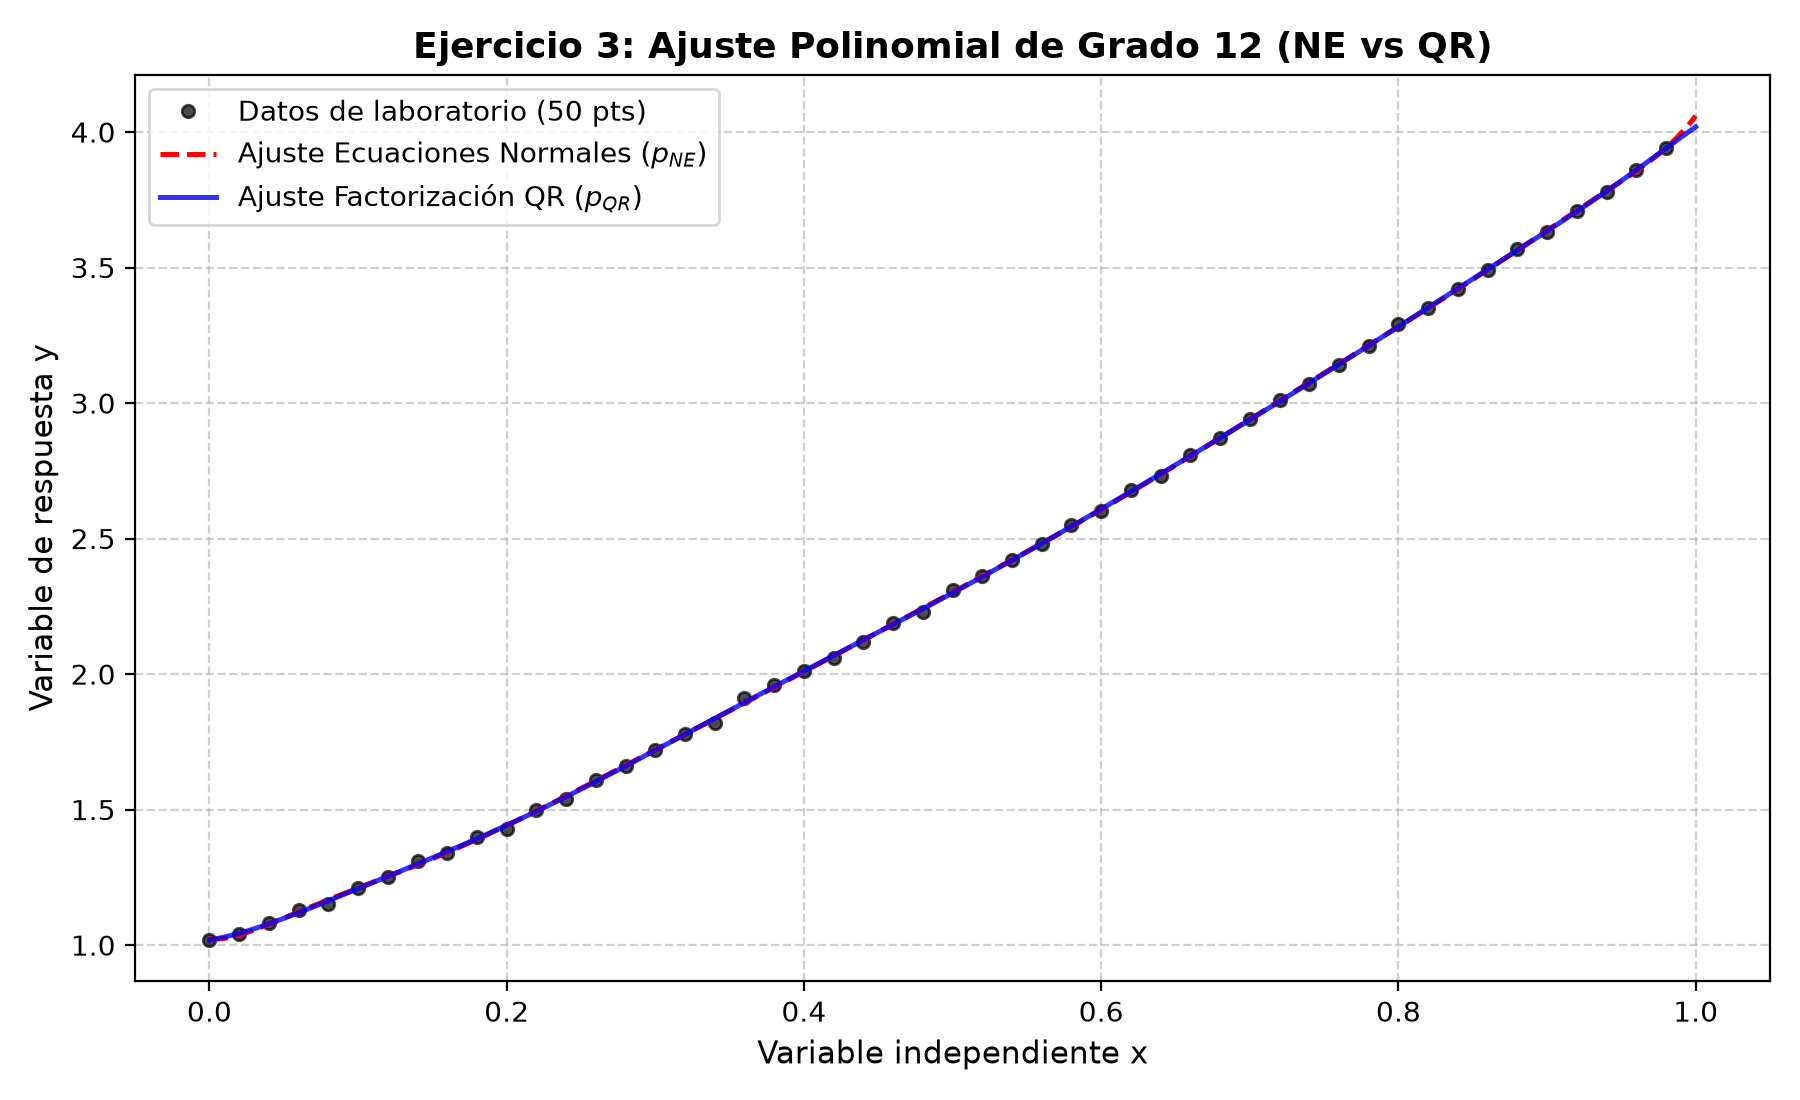
\includegraphics[width=0.68\textwidth]{fig_ejercicio3_minimos_cuadrados.png}
    \caption{Ajuste polinomial de grado 12 con Ecuaciones Normales y QR.}
\end{figure}

\subsection{e), f) y g) Condicionamiento de las matrices}
Calculando los números de condición en norma-2:
\begin{align*}
    \kappa(A) &\approx 7.76 \times 10^8 \\
    \kappa(A^T A) &\approx 3.13 \times 10^{17}
\end{align*}
Se comprueba que $\kappa(A^T A) \approx (\kappa(A))^2 \approx (7.76 \times 10^8)^2 \approx 6.02 \times 10^{17}$.
En precisión doble (IEEE 754 con 64 bits), el épsilon de máquina es aproximadamente $2.22 \times 10^{-16}$, por lo que el límite computable es $1/\varepsilon_{\text{mach}} \approx 4.5 \times 10^{15}$. Al superar este valor, la matriz $A^T A$ se vuelve numéricamente singular y el computador pierde todos los dígitos significativos en los modos más pequeños debido a errores de redondeo.

\subsection{Parte D. Perturbación de los datos}
Cambiamos el primer valor experimental en una cantidad muy pequeña: $y_0 \leftarrow y_0 + 10^{-6}$.
\begin{itemize}[leftmargin=*]
    \item En Ecuaciones Normales, la variación máxima en los coeficientes fue de $36.45$.
    \item En Factorización QR, la variación máxima fue de $8.63$.
\end{itemize}
En Ecuaciones Normales, una perturbación de $10^{-6}$ en un solo dato alteró los coeficientes en más de 36 unidades, lo que representa una amplificación del error de más de $3.6 \times 10^7$ veces.

\begin{figure}[h!]
    \centering
    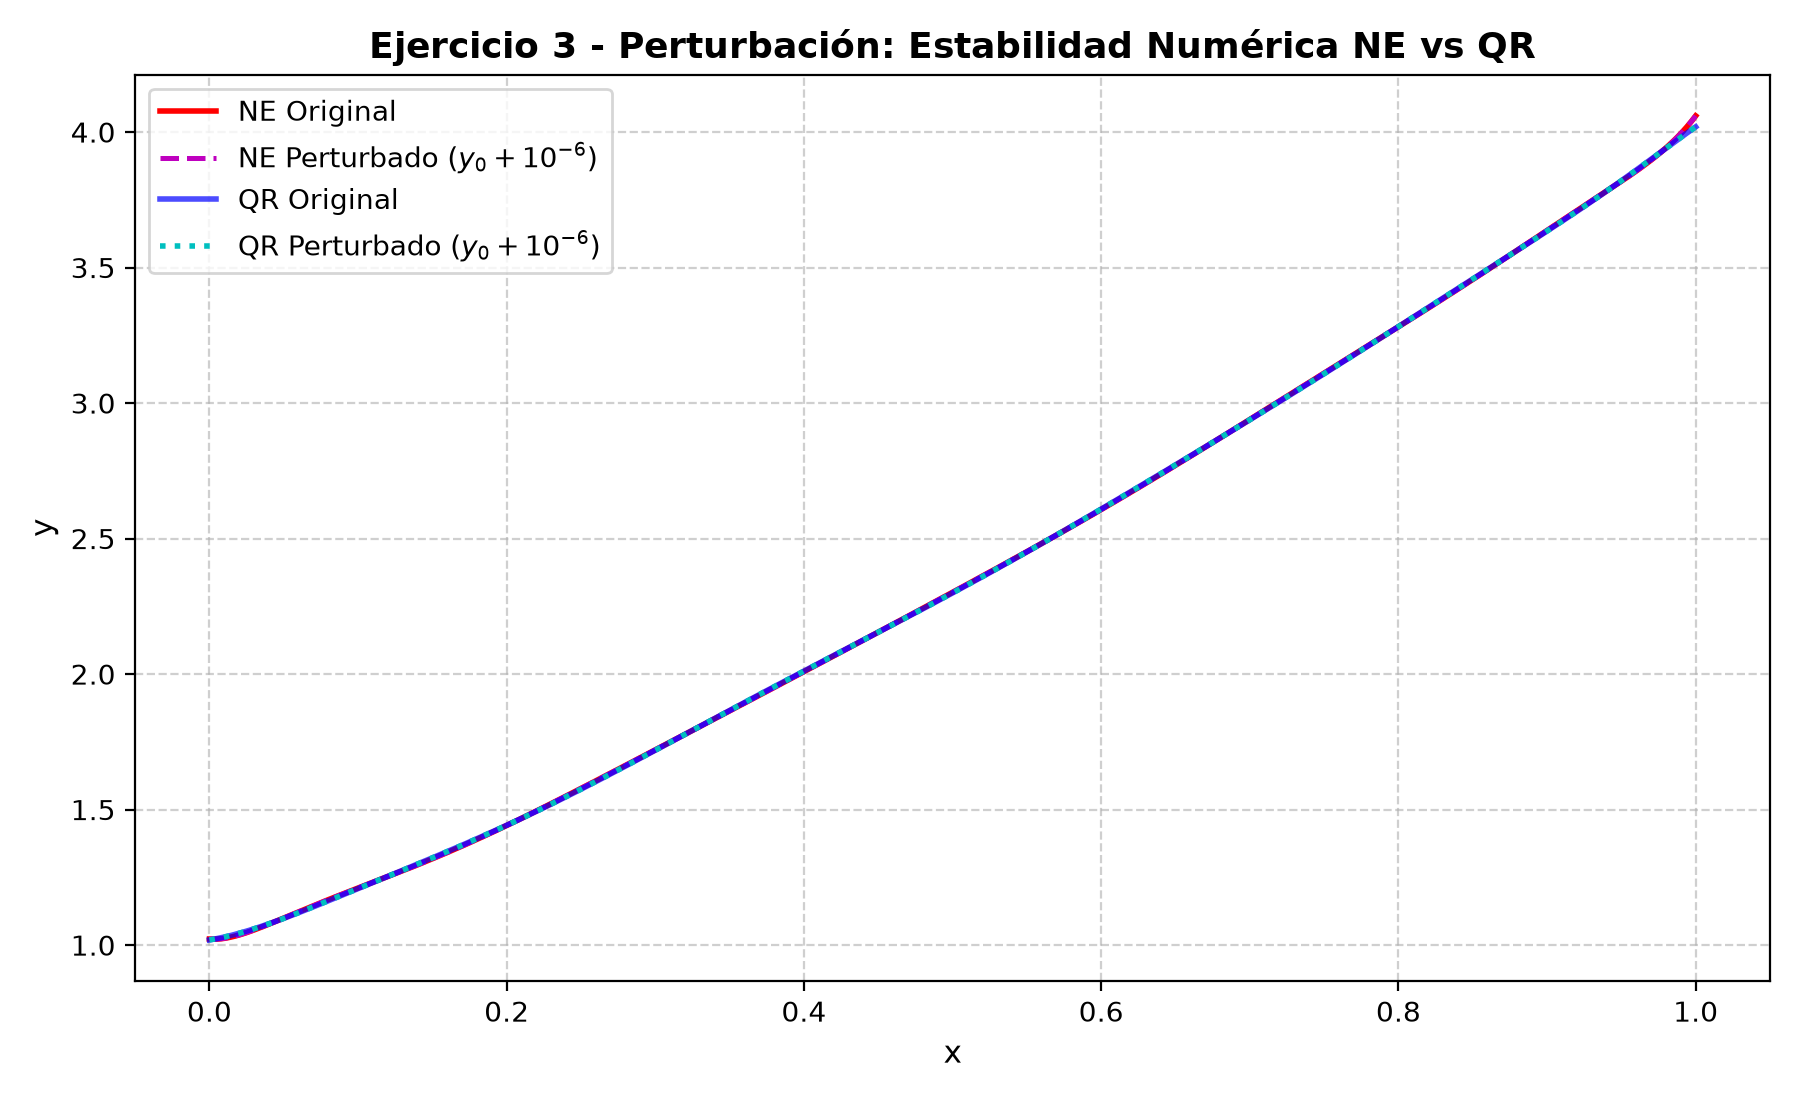
\includegraphics[width=0.68\textwidth]{fig_ejercicio3_perturbacion.png}
    \caption{Comparación del ajuste antes y después de perturbar $y_0$ en $10^{-6}$.}
\end{figure}

\subsection{Preguntas de análisis}
\begin{enumerate}[leftmargin=*]
    \item \textbf{¿Los dos métodos producen exactamente los mismos coeficientes?} \\
    No. Aunque matemáticamente representan el mismo problema, la aritmética finita del computador propaga los errores de redondeo de forma diferente, afectando mucho más a las ecuaciones normales.
    
    \item \textbf{Si los coeficientes son diferentes, ¿los residuos presentan una diferencia de la misma magnitud?} \\
    No. Los coeficientes difieren en órdenes de $10^5$, pero los residuos difieren en solo $10^{-3}$. Esto ocurre porque las funciones $x^k$ en el intervalo $[0, 1]$ tienen comportamientos muy parecidos; los grandes cambios con signos opuestos en los coeficientes se compensan entre sí y producen prácticamente la misma curva sobre los datos.
    
    \item \textbf{¿Qué relación observa entre el número de condicionamiento de $A$ y el de $A^T A$?} \\
    Se observa que $\kappa(A^T A) = (\kappa(A))^2$.
    
    \item \textbf{¿Por qué formar $A^T A$ puede empeorar las dificultades numéricas del problema?} \\
    Porque al elevar al cuadrado el número de condición se duplica la pérdida de cifras significativas. Al pasar de $10^8$ a $10^{17}$, se supera la precisión doble de 64 bits (16 dígitos decimales) y la matriz se vuelve numéricamente singular.
    
    \item \textbf{¿Qué método parece ser más estable para este problema?} \\
    La factorización QR. Al trabajar directamente sobre la matriz $A$ con transformaciones ortogonales (que conservan distancias y tienen número de condición 1), mantiene el condicionamiento original $\kappa(A) \approx 7.8 \times 10^8$ y evita que los errores numéricos se amplifiquen.
    
    \item \textbf{Explique por qué este ejemplo constituye un problema de mínimos cuadrados mal condicionado.} \\
    Porque se ajusta un polinomio de grado alto (12) usando la base de potencias $\{1, x, x^2, \dots, x^{12}\}$ en el intervalo $[0, 1]$. En ese rango, las columnas de la matriz de Vandermonde se vuelven casi colineales, generando valores singulares muy pequeños y haciendo que el problema sea muy sensible a cualquier perturbación o error de redondeo.
\end{enumerate}

\paragraph{Pregunta final:}
\textit{«Las ecuaciones normales y QR resuelven el mismo problema matemático, pero no necesariamente con la misma estabilidad numérica.»}

\medskip
En teoría matemática continua (con precisión infinita), ambos métodos son equivalentes porque encuentran la misma solución que minimiza la norma del residuo. Sin embargo, en un computador con aritmética finita:
\begin{itemize}[leftmargin=*]
    \item Las ecuaciones normales calculan $A^T A$, lo que eleva el número de condición al cuadrado y genera cancelaciones numéricas catastróficas.
    \item La factorización QR evita calcular $A^T A$ y opera mediante transformaciones ortogonales que conservan la norma euclidiana, manteniendo el condicionamiento original de la matriz.
\end{itemize}
Por esta razón, aunque resuelvan el mismo problema teórico, QR es mucho más estable y confiable en la práctica computacional.

\end{document}
